\documentclass[10pt,letterpaper]{article}
\usepackage{fontspec}
\usepackage{amsmath,amssymb}
\usepackage{graphicx}
\usepackage{xcolor}
\usepackage{tcolorbox}
\tcbuselibrary{skins}
\usepackage{geometry}
\usepackage{booktabs}
\usepackage{colortbl}
\usepackage{fancyhdr}
\usepackage{titlesec}
\usepackage[shortlabels,inline]{enumitem}
\usepackage{tabularx}
\usepackage{array}
\usepackage{multicol}
\usepackage{tikz}

\setmainfont{Times New Roman}
\setsansfont{Arial}

\geometry{
    paperwidth=612.05pt,
    paperheight=720.05pt,
    top=33.8pt,
    headheight=13pt,
    headsep=16pt,
    bottom=44pt,
    footskip=18pt,
    left=36pt,
    right=36pt,
    includehead
}

\definecolor{stewartcyan}{RGB}{0, 118, 186}
\definecolor{stewartred}{RGB}{218, 41, 28}
\definecolor{stewarttableheader}{RGB}{210, 224, 238}
\definecolor{stewarttablehead}{RGB}{210, 224, 238}
\definecolor{tableblue}{RGB}{210, 224, 238}
\definecolor{stewartlightblue}{RGB}{235, 243, 250}
\definecolor{stewartblue}{RGB}{0, 118, 186}
\definecolor{stewartgray}{RGB}{120, 120, 120}
\definecolor{stewartlightgray}{RGB}{240, 240, 240}
\definecolor{stewartpurple}{RGB}{85, 30, 95}
\definecolor{stewartpurplebg}{RGB}{243, 238, 245}
\definecolor{stewartpurpletext}{RGB}{85, 30, 95}
\definecolor{darkgray}{RGB}{40, 40, 40}

\pagestyle{fancy}
\fancyhf{}
\renewcommand{\headrulewidth}{0pt}

\providecommand{\makecell}[2][c]{\begin{tabular}[#1]{@{}c@{}}#2\end{tabular}}
\providecommand{\faDesktop}{\textbf{[Máy tính]}}
\providecommand{\casicon}{\textbf{\textsf{[CAS]}}}
\providecommand{\ticon}{\textbf{\textsf{[T]}}}
\providecommand{\captionof}[2]{\par\vspace{2pt}{\small\textbf{#1}: #2}\par}
\NewDocumentEnvironment{tasks}{o d()}{\begin{enumerate}}{\end{enumerate}}
\providecommand{\task}{\item}
\newenvironment{redframebox}{\begin{definitionbox}}{\end{definitionbox}}

\newtcolorbox{definitionbox}{
    colback=white,
    colframe=stewartred,
    arc=0mm,
    boxrule=0.9pt,
    left=3.5mm, right=3.5mm, top=3mm, bottom=3mm
}

\begin{document}
\fancyhead[L]{\textsf{\textbf{14}}\quad \textbf{\textsf{CHƯƠNG 1}}\quad \textsf{Hàm số và Mô hình}}
\fancyhead[R]{}

\noindent
\begin{minipage}[t]{0.26\textwidth}
    \vspace*{3.9cm}
    \begin{flushright}
        \textbf{\textsf{HÌNH 14}}
    \end{flushright}
    
    \vspace*{4.8cm}
    \begin{center}
        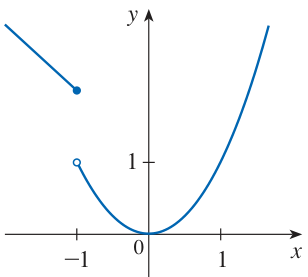
\includegraphics[width=0.88\linewidth]{images/p0049_fig15_clean.png}\\[2pt]
        {\small\textbf{\textsf{HÌNH 15}}}
    \end{center}
    
    \vspace*{1.2cm}
    \small
    \noindent\textit{Để ôn tập kỹ hơn về giá trị tuyệt đối, hãy xem Phụ lục A.}
\end{minipage}%
\hfill
\begin{minipage}[t]{0.71\textwidth}
    Chẳng hạn, parabol $x = y^2 - 2$ trong Hình 14(a) không phải là đồ thị của một hàm số của $x$ vì như ta thấy, có những đường thẳng đứng cắt parabol tại hai điểm. Tuy nhiên, parabol này lại chứa đồ thị của \emph{hai} hàm số của $x$. Chú ý rằng phương trình $x = y^2 - 2$ dẫn đến $y^2 = x + 2$, do đó $y = \pm\sqrt{x + 2}$. Như vậy, nửa trên và nửa dưới của parabol lần lượt là đồ thị của các hàm số $f(x) = \sqrt{x + 2}$ [từ Ví dụ 6(a)] và $g(x) = -\sqrt{x + 2}$ [xem các Hình 14(b) và (c)].

    \vspace{0.3cm}
    \noindent
    \centering
    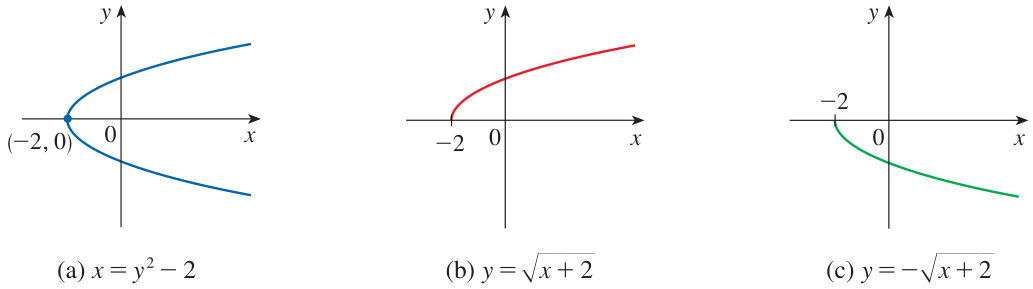
\includegraphics[width=\linewidth]{images/p0049_fig14_composite.png}

    \vspace{0.3cm}
    \raggedright
    Ta nhận thấy rằng nếu hoán đổi vai trò của $x$ và $y$, thì phương trình $x = h(y) = y^2 - 2$ \emph{thực sự} xác định $x$ là một hàm số theo biến $y$ (với $y$ là biến độc lập và $x$ là biến phụ thuộc). Đồ thị của hàm số $h$ chính là parabol ở Hình 14(a).

    \vspace{0.3cm}
    \noindent
    {\color{stewartcyan}\rule{1.2ex}{1.2ex}}\hspace{0.5em}\textbf{\textsf{\large Hàm số cho bởi nhiều công thức}}

    \vspace{0.15cm}
    Các hàm số trong bốn ví dụ sau đây được xác định bởi những công thức khác nhau trên các phần khác nhau của miền xác định. Những hàm số như vậy được gọi là \textbf{hàm số cho bởi nhiều công thức} (hay hàm từng khúc).

    \vspace{0.25cm}
    \noindent
    \textbf{\textsf{\color{stewartcyan}VÍ DỤ 7}}\quad Cho hàm số $f$ xác định bởi
    \[
    f(x) = \begin{cases}
    1 - x & \text{nếu } x \leqslant -1 \\
    x^2 & \text{nếu } x > -1
    \end{cases}
    \]
    Tính $f(-2)$, $f(-1)$, và $f(0)$, sau đó vẽ đồ thị hàm số.

    \vspace{0.15cm}
    \noindent
    \textbf{\textsf{\color{stewartcyan}LỜI GIẢI}}\quad Hãy nhớ rằng một hàm số là một quy tắc. Đối với hàm số cụ thể này, quy tắc được áp dụng như sau: Trước hết, hãy quan sát giá trị của biến đầu vào $x$. Nếu $x \leqslant -1$, thì giá trị của $f(x)$ là $1 - x$. Mặt khác, nếu $x > -1$, thì giá trị của $f(x)$ là $x^2$. Cần lưu ý rằng mặc dù sử dụng hai công thức khác nhau, $f$ vẫn chỉ là \emph{một} hàm số duy nhất, chứ không phải hai.
    \begin{align*}
    \text{Vì } -2 \leqslant -1, &\text{ nên ta có } f(-2) = 1 - (-2) = 3.\\
    \text{Vì } -1 \leqslant -1, &\text{ nên ta có } f(-1) = 1 - (-1) = 2.\\
    \text{Vì } 0 > -1, &\text{ nên ta có } f(0) = 0^2 = 0.
    \end{align*}
    Làm thế nào để ta vẽ đồ thị của $f$? Ta nhận thấy rằng nếu $x \leqslant -1$, thì $f(x) = 1 - x$, do đó phần đồ thị của $f$ nằm bên trái đường thẳng đứng $x = -1$ phải trùng với đường thẳng $y = 1 - x$, đường này có hệ số góc bằng $-1$ và tung độ gốc bằng $1$. Nếu $x > -1$, thì $f(x) = x^2$, do đó phần đồ thị của $f$ nằm bên phải đường thẳng $x = -1$ phải trùng với đồ thị của $y = x^2$, vốn là một parabol. Điều này cho phép ta phác thảo đồ thị như trong Hình 15. Điểm chấm đặc biểu thị điểm $(-1, 2)$ thuộc đồ thị; điểm chấm tròn rỗng biểu thị điểm $(-1, 1)$ bị loại trừ khỏi đồ thị. \hfill{\color{stewartcyan}$\blacksquare$}

    \vspace{0.25cm}
    Ví dụ tiếp theo về hàm số cho bởi nhiều công thức là hàm giá trị tuyệt đối. Nhắc lại rằng \textbf{giá trị tuyệt đối} của một số $a$, ký hiệu là $|a|$, là khoảng cách từ điểm $a$ đến $0$ trên trục số thực. Khoảng cách luôn mang giá trị không âm, vì vậy ta có
    \[
    |a| \geqslant 0 \qquad \text{với mọi số } a
    \]
\end{minipage}
\end{document}
